\section*{Seminár 12}
\subsection*{Téma}
Geometria IV -- kružnice vpísaná a opísaná trojuholníku

\subsection*{Ciele}
Precvičiť úlohy zamerané najmä na vlastnosti kružnice vpísanej a opísanej trojuholníku.

\subsection*{Úlohy a riešenia}
\begin{tcolorbox}[breakable,notitle,boxrule=0pt,colback=light-gray,colframe=light-gray]\ul{12.1} [57-II-1] Trojuholník $ABC$ spĺňa pri zvyčajnom označení dĺžok strán podmienku $a \leq b \leq c$. Vpísaná kružnica sa dotýka strán $AB$, $BC$ a $AC$ postupne v~bodoch $K$, $L$ a $M$. Dokážte, že z~úsečiek $AK$, $BL$ a $CM$ možno zostrojiť trojuholník práve vtedy, keď platí $b + c < 3a$.

\end{tcolorbox}

\rieh Označme $x = |AK| = |AM|$, $y = |BL| = |BK|$, $z = |CM| = |CL|$ (obr. 1) zhodné úseky dotyčníc z~jednotlivých vrcholov trojuholníka ku vpísanej kružnici.
\begin{center}
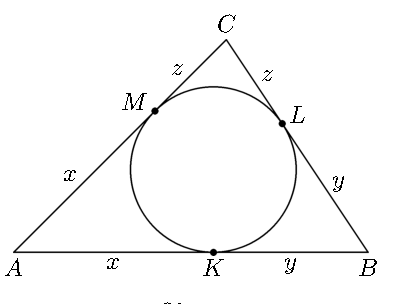
\includegraphics{obrazky/57K1}\\

Obr. 1
\end{center}
Zrejme
$$a= y + z, \ \ \ \ b = z~+ x, \ \ \ \ c = x + y. \ \ \ \ (1)$$
Z~uvedených rovností vidíme, že daná podmienka
$$b + c < 3a \ \ \ \ (2)$$
je ekvivalentná nerovnosti
$$x < y + z, \ \ \ \ (3)$$
čo je nutná podmienka existencie trojuholníka so stranami dĺžok $x$, $y$ a $z$.

Dosadením z~(1) do podmienok $b \leq c$ a $a \leq b$ zistíme, že $z \leq y$ a $y \leq x$. To znamená, že ďalšie dve trojuholníkové nerovnosti $y < z~+ x$ a $z < x + y$ sú automaticky splnené, takže nerovnosť (3), a tým aj (2) je podmienkou postačujúcou. Tým je tvrdenie úlohy dokázané.\\
\\
\kom Úloha využíva poznatok, že spojnice vrcholov a bodov dotyku so stredom vpísanej kružnice rozdelia trojuholník na tri dvojice zhodných trojuholníkov. Ten využijeme v~nasledujúcej úlohe aj domácej práci. Okrem toho, aj keď úloha nie je na výpočet nijako extrémne náročná, je študentov potrebné upozorniť, že dokazujú ekvivalenciu, takže nerovnosť zo zadania musí byť nielen podmienkou nutnou, ale aj postačujúcou.\\
\\
\begin{tcolorbox}[breakable,notitle,boxrule=0pt,colback=light-gray,colframe=light-gray]\ul{12.2} [61-S-2] Označme $S$ stred základne $AB$ daného rovnoramenného trojuholníka $ABC$. Predpokladajme, že kružnice vpísané trojuholníkom $ACS$, $BCS$ sa dotýkajú priamky $AB$ v~bodoch, ktoré delia základňu $AB$ na tri zhodné diely. Vypočítajte pomer $|AB| : |CS|$.

\end{tcolorbox}

\rieh Vďaka súmernosti podľa priamky $CS$ sa obe vpísané kružnice dotýkajú výšky $CS$ v~rovnakom bode, ktorý označíme $D$. Body dotyku týchto kružníc s~úsečkami $AS$, $BS$, $AC$, $BC$ označíme postupne $E$, $F$, $G$, $H$ (obr. 2). Pre vyjadrenie všetkých potrebných dĺžok ešte zavedieme označenie $x = |SD|$ a $y = |CD|$.
\begin{center}
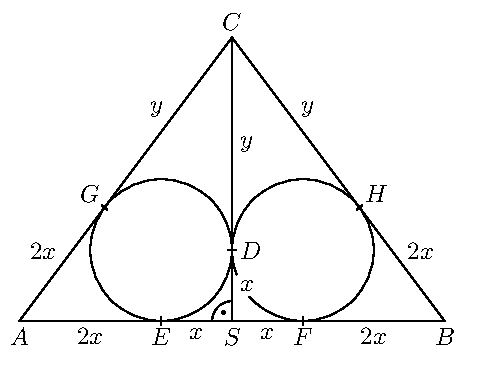
\includegraphics{obrazky/61S2}\\

Obr. 2
\end{center}
Vzhľadom na symetriu dotyčníc z~daného bodu k~danej kružnici platia rovnosti
$$|SD| = |SE| = |SF| = x \ \ \ \ \text{a} \ \ \ \ |CD| = |CG| = |CH| = y.$$
Úsečka $EF$ má preto dĺžku $2x$, ktorá je podľa zadania zároveň dĺžkou úsečiek $AE$ a $BF$, a teda aj dĺžkou úsečiek $AG$ a $BH$ (opäť vďaka symetrii dotyčníc). Odtiaľ už bezprostredne vyplývajú rovnosti
$$|AB| = 6x, \ \ \ \ |AC| = |BC| = 2x + y \ \ \ \ \text{a} \ \ \ \  |CS| = x + y.$$

Závislosť medzi dĺžkami $x$ a $y$ zistíme použitím Pytagorovej vety pre pravouhlý trojuholník $ACS$ (s~odvesnou $A$ dĺžky $3x$):
$$(2x + y)^2= (3x)^2+ (x + y)^2.$$
Roznásobením a ďalšími úpravami odtiaľ dostaneme ($x$ a $y$ sú kladné hodnoty)
\begin{align*}
4x^2+ 4xy + y^2 &= 9x^2+ x^2+ 2xy + y^2,\\
2xy & = 6x^2,\\
y &= 3x.
\end{align*}
Hľadaný pomer tak má hodnotu
$$|AB| : |CS| = 6x : (x + y) = 6x : 4x = 3 : 2.$$
Poznamenajme, že prakticky rovnaký postup celého riešenia možno zapísať aj pri štandardnom označení $c = |AB|$ a $v = |CS|$. Keďže podľa zadania platí $|AE| =\frac{1}{3}c$, a teda $|SE| =\frac{1}{6}c$, z~rovnosti $|SD| = |SE|$ vyplýva $|CD| = |CS|-|SD| = v-\frac{1}{6}c$, odkiaľ
$$|AC| = |AG| + |CG| = |AE| + |CD| =\tfrac{1}{3}c + (v-\tfrac{1}{6}c) = v~+\tfrac{1}{6}c,$$
takže z~Pytagorovej vety pre trojuholník $ACS$,
$$(v +\tfrac{1}{6}c)^2= (\tfrac{1}{2}c)^2+ v^2,$$
vychádza $3v = 2c$, čiže $c : v~= 3 : 2$.\\
\\
\kom Úloha vychádza z~poznatku, ktorý si študenti osvojili v~úlohe predchádzajúcej a pridáva k~nemu ešte prácu s~Pytagorovou vetou a manipuláciu s~algebraickými výrazmi, takže tvorí prirodzené pokračovanie úlohy predchádzajúcej.\\
\\
\begin{tcolorbox}[breakable,notitle,boxrule=0pt,colback=light-gray,colframe=light-gray]\ul{12.3} [62-S-1] Danému rovnostrannému trojuholníku vpíšme a opíšme kružnicu. Označme $S$ obsah vzniknutého medzikružia a $T$ obsah kruhu, ktorého priemer je zhodný s~dĺžkou strany daného trojuholníka. Ktorý z~obsahov $S$, $T$ je väčší? Svoju odpoveď zdôvodnite.

\end{tcolorbox}

\rieh Ukážeme, že sa oba obsahy rovnajú. Označme $A$, $B$, $C$ vrcholy daného trojuholníka a $r$ a $R$ zodpovedajúce polomery jeho vpísanej a opísanej kružnice; dĺžku jeho strany označme $a$. Obe uvedené kružnice majú spoločný stred $S$. Označme ešte $P$ bod dotyku vpísanej kružnice so stranou $AB$. Keďže trojuholník $ABC$ je rovnostranný, je $P$ zároveň stredom strany $AB$. Použitím Pytagorovej vety v~pravouhlom trojuholníku $PSB$ dostávame
$$R^2 - r^2=  (\tfrac{1}{2}a)^2,$$
čo je ekvivalentné s~dokazovaným tvrdením $S = \pi (R^2 - r^2) = \pi \big( \frac{1}{2}a\big)^2= T$.\\
\\
\textit{Poznámka.} Rovnostranný trojuholník so stranou $a$ má výšku veľkosti $v = \frac{1}{2}a \sqrt{3}$, takže skúmané polomery sú $R =\frac{2}{3}v \big(=\frac{1}{3}a\sqrt{3}\big)$ a $r =\frac{1}{3}v \big(=\frac{1}{6}a\sqrt{3}\big)$, a preto
$$S = \pi ( R^2 - r^2) = \pi \big( \tfrac{4}{9} -\tfrac{1}{9})v^2= \pi \cdot \tfrac{1}{3}\cdot\tfrac{3}{4}a^2= \pi \big( \tfrac{1}{2}a\big)^2= T.$$
\\
\kom Úloha je relatívne jednoduchá, využíva znalosť o~bode dotyku vpísanej kružnice a taktiež pripravuje študentov na nasledujúcu zložitejšiu analýzu. \\
\\
\begin{tcolorbox}[breakable,notitle,boxrule=0pt,colback=light-gray,colframe=light-gray]\ul{12.4} [61-I-5] Daný je rovnoramenný trojuholník so základňou dĺžky $a$ a ramenami dĺžky $b$. Pomocou nich vyjadrite polomer $R$ kružnice opísanej a polomer $r$ kružnice vpísanej tomuto trojuholníku. Potom ukážte, že platí $R \geq 2r$ a zistite, kedy nastane rovnosť.

\end{tcolorbox}

\rieh Označme $S$ stred základne $BC$ daného rovnoramenného trojuholníka $ABC$, $O$ stred jeho opísanej kružnice, $M$ stred vpísanej kružnice a $P$ pätu kolmice z~bodu $M$ na rameno $AC$ (obr. 3).
\begin{center}
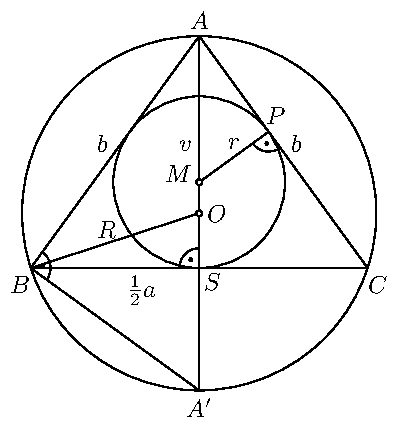
\includegraphics{obrazky/61D5}

Obr. 3
\end{center}
Z~pravouhlého trojuholníka $BSA$ pomocou Pytagorovej vety vyjadríme veľkosť $v$ výšky $AS$, pričom v~pravouhlom trojuholníku $BSO$ s~preponou dĺžky $R$ pre odvesnu $OS$ platí $|OS| =||AS|-|AO|| = |v-R|$ (musíme si uvedomiť, že v~tupouhlom trojuholníku $ABC$ bude bod $S$ ležať medzi bodmi $A$ a $O$!). Dostávame tak dve rovnosti
\begin{align*}
v^2 &= b^2 -\frac{a^2}{4},\\
R^2 &= \frac{a^2}{4}+ (v~-R)^2;
\end{align*}
ich sčítaním vyjde
$$v^2+ R^2= b^2 + (v~- R)^2,\ \ \ \ \text{čiže} \ \ \ \  b^2= 2vR.$$
Dosadením z~prvej rovnice $v =\frac{1}{2}\sqrt{4b^2- a^2}$ do poslednej rovnosti dostaneme hľadaný vzorec pre $R$.

Dodajme, že rovnosť $b^2 = 2vR$, ktorú sme práve odvodili a z~ktorej už ľahko vyplýva vzorec pre polomer $R$, je Euklidovou vetou o~odvesne $AB$ pravouhlého trojuholníka $ABA'$ s~preponou $AA'$, ktorá je priemerom kružnice opísanej trojuholníku $ABC$ (obr. 3).

Nájdený vzorec pre polomer $R$ zapíšeme prehľadne spolu s~druhým hľadaným vzorcom pre polomer $r$, ktorého odvodeniu sa ešte len budeme venovať:
$$R =\frac{\sqrt{b^2}}{\sqrt{4b^2 - a^2}}\ \ \ \ \text{a}\ \ \ \  r = \frac{a\sqrt{4b^2-a^2}}{2(a+2b)}.\ \ \ \  (\ast)$$
Druhý zo vzorcov ($\ast$) sa dá získať okamžite zo známeho vzťahu $r = 2S/(a + b + c)$ pre polomer $r$ kružnice vpísanej do trojuholníka so stranami $a$, $b$, $c$ a obsahom $S$;
v~našom prípade stačí len dosadiť $b = c$ a $2S = av$, kde $v = \frac{1}{2}\sqrt{4b^2 - a^2}$ podľa úvodnej časti riešenia.

Ďalšie dva spôsoby odvodenia druhého zo vzorcov ($\ast$) založíme na úvahe o~pravouhlom trojuholníku $AMP$, ktorého strany majú dĺžky
$$|AM| = v~-r, \ \ \ \ |MP| = r, \ \ \ \ |AP| = |AC| - |PC| = b - |SC| = b - \frac{a}{2}.$$
Pre tento trojuholník môžeme napísať Pytagorovu vetu alebo využiť jeho podobnosť s~trojuholníkom $ACS$, konkrétne zapísať rovnosť sínusov ich spoločného uhla pri vrchole $A$. Podľa toho dostaneme rovnice
$$(v - r)^2= r^2+\big(b -\frac{a}{2}\big)^2, \ \ \ \ \text{resp.} \ \ \ \ \frac{r}{v-r}=  \frac{\frac{1}{2}a}{b},$$
ktoré sú obidve lineárne vzhľadom na neznámu $r$ a majú riešenie
$$r = \frac{v}{2}-\frac{1}{2v}\cdot \big( b - \frac{a}{2} \big)^2, \ \ \ \ \text{resp.}\ \ \ \  r=
\frac{av}{a+2b}.$$
Po dosadení za $v$ v~oboch prípadoch dostaneme hľadaný vzorec pre $r$. V~druhom prípade
je to zrejmé, v~prvom to ukážeme:
$$r =\frac{v}{2}  - \frac{1}{2v} \cdot \big(b \frac{a}{2}\big)^2= \frac{v^2 - b^2 + ab \frac{1}{4}a^2}{2v}=\frac{2ab - a^2}{4v}=\frac{a(2b - a)}{2\sqrt{(2b -a)(2b + a)}}=\frac{2\sqrt{2b-a}}{2\sqrt{2b-a}}= \\ =\frac{a \sqrt{4b^2 -a^2}}{2(a + 2b)}.$$

Ešte ostáva dokázať nerovnosť $R \geq 2r$. Využijeme na to odvodené vzorce ($\ast$), z~ktorých dostávame (pripomíname, že $2b > a > 0$)
$$ \frac{R}{2r}= R \cdot \frac{1}{2r}=\frac{b^2}{\sqrt{4b^2-a^2}}\cdot \frac{a+2b}{a \sqrt{4b^2-a^2}}=\frac{b^2}{a(2b-a)}.$$
Nerovnosť $R \geq 2r$ teda platí práve vtedy, keď $b^2\geq a(2b -a)$. Posledná nerovnosť je však ekvivalentná s~nerovnosťou $(a - b)^2\geq 0$, ktorej platnosť je už zrejmá. Tým je dôkaz nerovnosti $R \geq 2r$ hotový. Navyše vidíme, že rovnosť v~nej nastane jedine v~prípade, keď $(a - b)^2 = 0$, čiže $a = b$, teda práve vtedy, keď je pôvodný trojuholník nielen rovnoramenný, ale dokonca rovnostranný.\\
\\
\kom Úloha poskytuje mnoho prístupov k~riešeniu a bude zaujímavé nechať študentov porovnať ich výsledky. Spája tiež zistenia z~predchádzajúcich úloh, v~niektorých prípadoch študenti využijú Euklidovu vetu a nezaobídu sa ani bez zručnej manipulácie s~algebraickými výrazmi. \\
\\
\begin{tcolorbox}[breakable,notitle,boxrule=0pt,colback=light-gray,colframe=light-gray]\ul{12.5} [63-I-2]  V~rovine sú dané body $A$, $P$, $T$ neležiace na jednej priamke. Zostrojte trojuholník $ABC$ tak, aby $P$ bola päta jeho výšky z~vrcholu $A$ a $T$ bod dotyku strany $AB$ s~kružnicou jemu vpísanou. Uveďte diskusiu o~počte riešení vzhľadom na polohu daných bodov.

\end{tcolorbox}

\rieh Vrchol $B$ je určený polpriamkou $AT$ a kolmicou $p$ na výšku $AP$ v~bode $P$ (obr. 4), na ktorej leží strana $BC$. Pritom bod $T$ musí byť vnútorným bodom úsečky $AB$. Stred $S$ kružnice vpísanej trojuholníku $ABC$ potom dostaneme ako priesečník kolmice $q$
\begin{center}
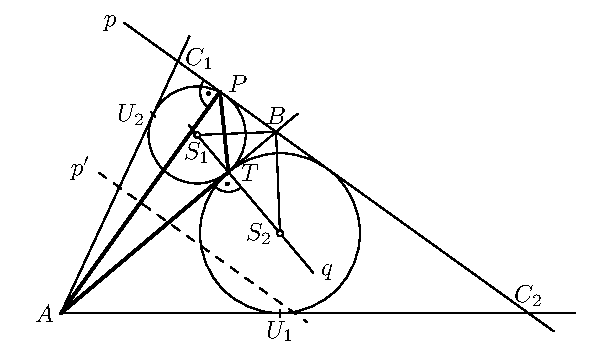
\includegraphics{obrazky/63D2}\\

Obr. 4
\end{center}
na priamku $AT$ v~bode $T$ s~osou uhla ohraničeného priamkou $p$ a polpriamkou $BA$. Jej polomer bude mať veľkosť $|ST|$.

Ostáva zostrojiť vrchol $C$ hľadaného trojuholníka $ABC$. Ten bude ležať jednak na priamke $p$, jednak na druhej dotyčnici vpísanej kružnice z~vrcholu $A$, ktorá je súmerne združená so stranou $AB$ podľa priamky $AS$. Stačí teda zostrojiť bod $U$ dotyku strany $AC$ s~kružnicou vpísanou ako obraz bodu $T$ v~uvedenej osovej súmernosti.

Odtiaľ vyplýva \textit{konštrukcia}:
\begin{enumerate}
\item $p$: $P \in p$ a $p \perp AP$;
\item $B$: $B \in AT \cap p$, bod $B$ musí ležať na polpriamke $AT$ za bodom $T$;
\item $q$: $T \in q$ a $q \perp AT$;
\item $u_1$, $u_2$: dve (navzájom kolmé) osi rôznobežiek $AB$, $p$;
\item $S_1$, $S_2$: $S_1 \in q \cap u_1$, $S_2 \in q \cap u_2$;
\item $U_1$, $U_2$: obrazy bodu $T$ v~súmernostiach podľa priamok $AS_1$ a $AS_2$;
\item $C_1$, $C_2$: priesečníky priamky $p$ s~polpriamkami $AU_1$ a $AU_2$;
\item trojuholníky $ABC_1$ a $ABC_2$.
\end{enumerate}
\textit{Diskusia.} Bod $B$ konštruovaný v~2. kroku existuje, len ak uhol $PAT$ je ostrý (inak ani polpriamka $AT$ nepretne priamku $p$) a zároveň bod $T$ leží vnútri polroviny $pA$, čo je ekvivalentné s~tým, že aj uhol $APT$ je ostrý. Body $S_1$, $S_2$ existujú vždy a sú rôzne, lebo ležia v~opačných polrovinách určených priamkou $AB$. Kružnica vpísaná leží celá v~trojuholníku $ABC$, a teda i v~páse určenom priamkou $p$ a priamkou s~ňou rovnobežnou, ktorá prechádza vrcholom $A$, takže stred $S$ vpísanej kružnice musí padnúť do pásu tvoreného priamkou $p$ a priamkou $p'$ s~ňou rovnobežnou, ktorá rozpoľuje výšku $AP$. V~takom prípade dotyčnica ku kružnici $(S; |ST|)$ (súmerne združená s~dotyčnicou $AB$ podľa priamky $AS$) určite pretne priamku $p$ v~hľadanom vrchole $C$.

Diskusiu zhrnieme takto: Ak pre vnútorné uhly trojuholníka $APT$ platí $|\ma PAT| \geq 90^\circ$ alebo $|\ma APT| \geq 90^\circ$, nemá úloha riešenie. Ak platí $|\ma PAT| < 90^\circ$ a zároveň $|\ma APT| < 90^\circ$, je počet riešení 0 až 2 podľa toho, koľko zo zostrojených bodov $S_1$ a $S_2$ leží medzi rovnobežkami $p$ a $p'$.\\
\\
\kom V~posledných rokoch sa v~MO nevyskytlo veľké množstvo konštrukčných úloh. Napriek tomu však považujeme za dôležité vyriešiť so študentmi aspoň jeden takýto problém a poukázať na to, že zostrojením vyhovujúceho útvaru riešenie úlohy nekončí a je potrebné uviesť aj diskusiu, ktorá je častokrát aspoň tak náročná ako vhodná konštrukcia. Zaradenie úlohy v~tomto seminári považujeme za vhodné tiež preto, lebo úloha využíva vlastnosti kružnice vpísanej, a tak so cťou uzavrie toto seminárne stretnutie.

\subsection*{Domáca práca}
\begin{tcolorbox}[breakable,notitle,boxrule=0pt,colback=light-gray,colframe=light-gray]\ul{12.6} [59-I-4] Kružnica $k(S; r)$ sa dotýka priamky $AB$ v~bode $A$. Kružnica $l(T; s)$ sa dotýka priamky $AB$ v~bode $B$ a pretína kružnicu k~v~krajných bodoch $C$, $D$ jej priemeru. Vyjadrite dĺžku a úsečky $AB$ pomocou polomerov $r$, $s$. Dokážte ďalej, že priesečník $M$ priamok $CD$, $AB$ je stredom úsečky $AB$.

\end{tcolorbox}

\rieh Keďže kružnica $l$ má ako tetivu priemer $CD$ kružnice $k$ a dané kružnice nie sú totožné, platí pre ich polomery nerovnosť $s > r$. Ak označíme $P$ pätu kolmice z~bodu $S$ na úsečku $BT$ (obr. 5), tak z~Pytagorovej vety pre pravouhlé trojuholníky
\begin{center}
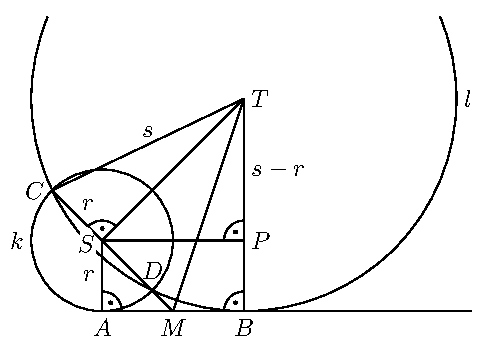
\includegraphics{obrazky/59D4}\\

Obr. 5
\end{center}
$CST$ a $SPT$ vyplýva
$$|ST|^2 = s^2 - r^2\ \ \ \ \text{a} \ \ \ \  |ST|^2 = |SP|^2 + (s~-r)^2. \ \ \ \  (1)$$
Odtiaľ pre veľkosť úsečky $SP$ vychádza
$$|SP|^2 = (s^2 - r^2 ) - (s~- r)^2 = 2r(s - r).$$
A~keďže $ABPS$ je pravouholník, dostávame
$$|AB| = |SP| =\sqrt{2r(s - r)}.$$

Z~pravouhlých trojuholníkov $AMS$ a $MTS$ ďalej podľa prvej rovnosti v~(1) vyplýva
$$|AM|^2 = |SM|^2 - r^2 = |MT|^2- |ST|^2 - r^2 = |MT|^2 -s^2,$$
pritom z~pravouhlého trojuholníka $MBT$ máme
$$|BM|^2 = |MT|^2 - s^2.$$
Preto $|AM| = |BM|$ a bod $M$ je teda stredom úsečky $AB$.

\textit{Poznámka.} Záver, že $M$ je stredom úsečky $AB$, vyplýva okamžite aj z~mocnosti bodu $M$ k~obom kružniciam (bod $M$ leží na tzv. chordále oboch kružníc). Tieto pojmy sú však pre súťažiacich kategórie C zväčša neznáme a nebudú nutné ani pre riešenia ďalších súťažných kôl.\\
\\
\begin{tcolorbox}[breakable,notitle,boxrule=0pt,colback=light-gray,colframe=light-gray]\ul{12.7} [61-I-2] Dĺžky strán trojuholníka sú v~metroch vyjadrené celými číslami. Určte ich, ak má trojuholník obvod 72\,m a ak je najdlhšia strana trojuholníka rozdelená bodom dotyku vpísanej kružnice v~pomere $3 : 4.$

\end{tcolorbox}

\rieh Využijeme všeobecný poznatok, že body dotyku vpísanej kružnice delia hranicu trojuholníka na šesť úsečiek, a to tak, že každé dve z~nich, ktoré vychádzajú z~toho istého vrcholu trojuholníka, sú zhodné. (Dotyčnice z~daného bodu k~danej kružnici sú totiž súmerne združené podľa spojnice daného bodu so stredom danej kružnice.)

V~našej úlohe je najdlhšia strana trojuholníka rozdelená na úseky, ktorých dĺžky označíme $3x$ a $4x$; dĺžku úsekov z~vrcholu oproti najdlhšej strane označíme $y$ (obr. 6). Strany trojuholníka majú teda dĺžky $7x$, $4x + y$ a $3x + y$, kde $x$, $y$ sú neznáme kladné čísla (dĺžky berieme bez jednotiek). Ak má byť $7x$ dĺžka najdlhšej strany, musí platiť $7x > 4x + y$, čiže $3x > y$. Zdôraznime, že hľadané čísla $x, y$ nemusia byť nutne celé, podľa zadania to však platí o~číslach $7x$, $4x + y$ a $3x + y$.
\begin{center}
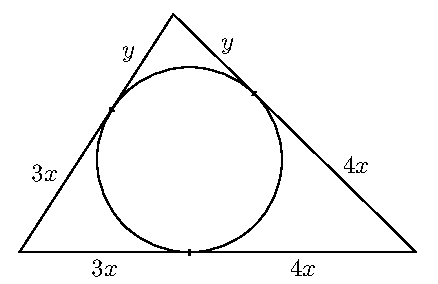
\includegraphics{obrazky/61D1}\\

Obr. 6
\end{center}
Údaj o~obvode trojuholníka zapíšeme rovnosťou
$$72 = 7x + (3x + y) + (4x + y), \ \ \ \ \text{čiže} \ \ \ \ 36 = 7x + y.$$
Pretože $7x$ je celé číslo, je celé i číslo $y = 36 - 7x$; a pretože podľa zadania i čísla $4x + y$ a $3x + y$ sú celé, je celé i číslo $x = (4x + y) - (3x + y)$. Preto od tohto okamihu už hľadáme dvojice celých kladných čísel $x$, $y$, pre ktoré platí
$$3x > y \ \ \ \ \text{a}  \ \ \ \ 7x + y = 36.$$
Odtiaľ vyplýva $7x < 36 < 7x + 3x = 10x$, teda $x \leq 5$ a súčasne $x \geq 4$.

Pre $x = 4$ je $y = 8$ a $(7x, 4x+y, 3x+y) = (28, 24, 20)$, pre $x = 5$ je $y = 1$ a $(7x, 4x+ + y, 3x + y) = (35, 21, 16)$. Strany trojuholníka sú teda $(28, 24, 20)$ alebo $(35, 21, 16)$. (Trojuholníkové nerovnosti sú zrejme splnené.)

